\documentclass[10pt,twocolumn,letterpaper]{article}

%%%%%%%%% PAPER TYPE  - PLEASE UPDATE FOR FINAL VERSION
% \usepackage{cvpr}              % To produce the CAMERA-READY version
\usepackage[cvprfinal]{cvpr}      % To produce the REVIEW version
\usepackage{hyperref}
% \usepackage[pagenumbers]{cvpr} % To force page numbers, e.g. for an arXiv version

% Import additional packages in the preamble file, before hyperref
%
% --- inline annotations
%
\usepackage[dvipsnames]{xcolor}
\newcommand{\red}[1]{{\color{red}#1}}
\newcommand{\todo}[1]{{\color{red}#1}}
\newcommand{\TODO}[1]{\textbf{\color{red}[TODO: #1]}}
% --- disable by uncommenting  
% \renewcommand{\TODO}[1]{}
% \renewcommand{\todo}[1]{#1}



% It is strongly recommended to use hyperref, especially for the review version.
% hyperref with option pagebackref eases the reviewers' job.
% Please disable hyperref *only* if you encounter grave issues, 
% e.g. with the file validation for the camera-ready version.
%
% If you comment hyperref and then uncomment it, you should delete *.aux before re-running LaTeX.
% (Or just hit 'q' on the first LaTeX run, let it finish, and you should be clear).
\definecolor{cvprblue}{rgb}{0.21,0.49,0.74}
\usepackage[pagebackref,breaklinks,colorlinks,citecolor=cvprblue]{hyperref}

%%%%%%%%% PAPER ID  - PLEASE UPDATE
\def\paperID{*****} % *** Enter the Paper ID here
\def\confName{CVPR}
\def\confYear{2024}

%%%%%%%%% TITLE - PLEASE UPDATE
\title{Visual Question Answering Using BLIP}

%%%%%%%%% AUTHORS - PLEASE UPDATE
\author{
Shreyas Kabra\\
2021563\\
{\tt\small shreyas21563@iiitd.ac.in}
\and
Ritwik Harit\\
2021557\\
{\tt\small ritwik21557@iiitd.ac.in}
\and
Vasan Vohra\\
2021572\\
{\tt\small vasan21572@iiitd.ac.in}
}

\begin{document}
\maketitle
\begin{abstract}
Our study evaluates the BLIP model's performance in Visual Question Answering (VQA) across three datasets. Using WUPS Score, BERT Score, VQA Score, etc, we assess its ability to generalise and predict answers accurately. We provide insights into metric selection, rationale, and advantages/disadvantages. This analysis informs on the BLIP model's capabilities in VQA, guiding future research.
\end{abstract}    
\section{Introduction}
\label{sec:intro}

In the realm of Computer Vision and Natural Language Processing, Visual Question Answering (VQA) presents a formidable challenge, demanding a deep comprehension of both linguistic nuances and visual semantics. This task involves an AI system analysing an image alongside a corresponding natural language query and then generating a coherent textual response. Our project endeavours to assess the efficacy of the BLIP model across three distinct datasets (VQA v2.0 dataset (training), VQA v2.0 dataset (validation) and DAQUAR - DAtaset for QUestion Answering on Real-world images), aiming to ascertain its ability to generalise and accurately predict answers. To comprehensively evaluate the model's performance, we adopt a diverse set of evaluation metrics, including WUPS Score, BERT Score, and VQA Score, etc. Each metric offers unique insights into the model's capabilities, and we delve into the rationale behind their selection, along with their respective advantages and disadvantages, to provide a comprehensive evaluation framework.

\begin{figure}[htbp]
  \centering
   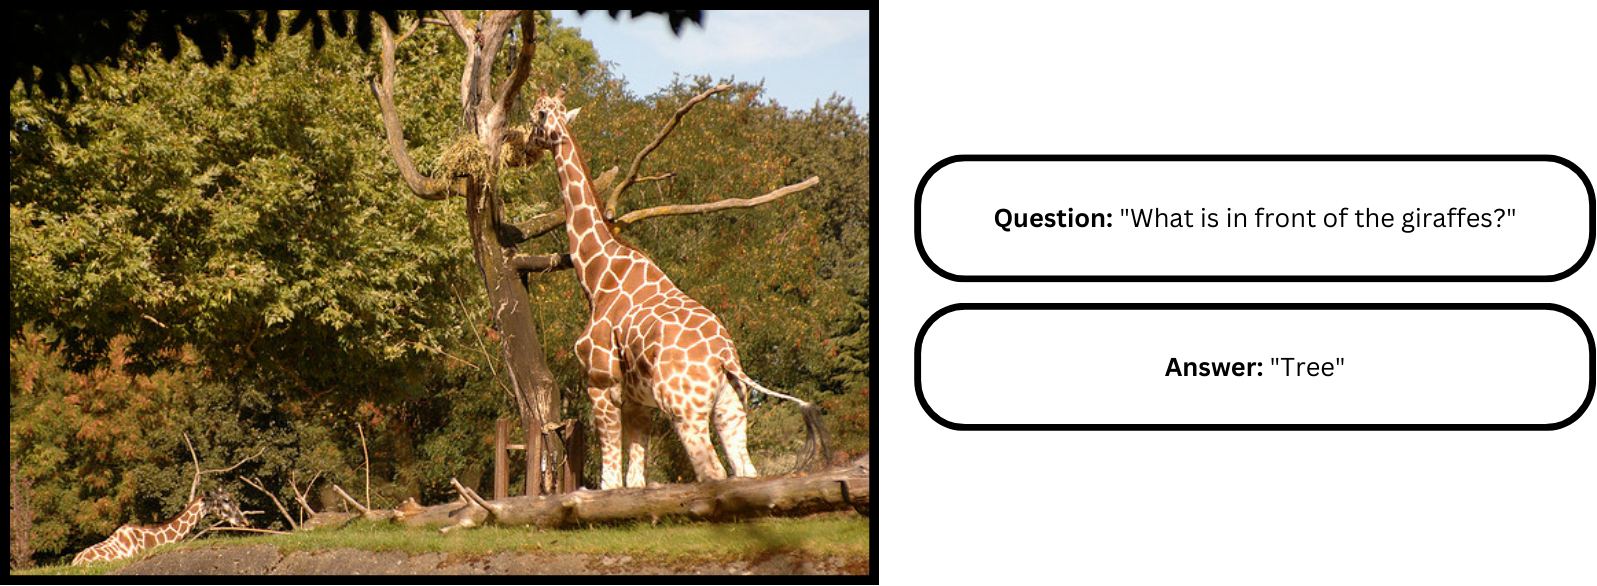
\includegraphics[width=\linewidth]{sec/Images/image1.png}
   \caption{Random examples from the VQA v2 training dataset}
   \label{fig:onecol}
\end{figure}

%-------------------------------------------------------------------------
% \subsection{Language}

% All manuscripts must be in English.

% \subsection{Dual submission}

% Please refer to the author guidelines on the \confName\ \confYear\ web page for a
% discussion of the policy on dual submissions.

% \subsection{Paper length}
% Papers, excluding the references section, must be no longer than eight pages in length.
% The references section will not be included in the page count, and there is no limit on the length of the references section.
% For example, a paper of eight pages with two pages of references would have a total length of 10 pages.
% {\bf There will be no extra page charges for \confName\ \confYear.}

% Overlength papers will simply not be reviewed.
% This includes papers where the margins and formatting are deemed to have been significantly altered from those laid down by this style guide.
% Note that this \LaTeX\ guide already sets figure captions and references in a smaller font.
% The reason such papers will not be reviewed is that there is no provision for supervised revisions of manuscripts.
% The reviewing process cannot determine the suitability of the paper for presentation in eight pages if it is reviewed in eleven.

% %-------------------------------------------------------------------------
% \subsection{The ruler}
% The \LaTeX\ style defines a printed ruler which should be present in the version submitted for review.
% The ruler is provided in order that reviewers may comment on particular lines in the paper without circumlocution.
% If you are preparing a document using a non-\LaTeX\ document preparation system, please arrange for an equivalent ruler to appear on the final output pages.
% The presence or absence of the ruler should not change the appearance of any other content on the page.
% The camera-ready copy should not contain a ruler.
% (\LaTeX\ users may use options of \texttt{cvpr.sty} to switch between different versions.)

% Reviewers:
% note that the ruler measurements do not align well with lines in the paper --- this turns out to be very difficult to do well when the paper contains many figures and equations, and, when done, looks ugly.
% Just use fractional references (\eg, this line is $087.5$), although in most cases one would expect that the approximate location will be adequate.


% \subsection{Paper ID}
% Make sure that the Paper ID from the submission system is visible in the version submitted for review (replacing the ``*****'' you see in this document).
% If you are using the \LaTeX\ template, \textbf{make sure to update paper ID in the appropriate place in the tex file}.


% \subsection{Mathematics}

% Please number all of your sections and displayed equations as in these examples:
% \begin{equation}
%   E = m\cdot c^2
%   \label{eq:important}
% \end{equation}
% and
% \begin{equation}
%   v = a\cdot t.
%   \label{eq:also-important}
% \end{equation}
% It is important for readers to be able to refer to any particular equation.
% Just because you did not refer to it in the text does not mean some future reader might not need to refer to it.
% It is cumbersome to have to use circumlocutions like ``the equation second from the top of page 3 column 1''.
% (Note that the ruler will not be present in the final copy, so is not an alternative to equation numbers).
% All authors will benefit from reading Mermin's description of how to write mathematics:
% \url{http://www.pamitc.org/documents/mermin.pdf}.

% \subsection{Blind review}

% Many authors misunderstand the concept of anonymizing for blind review.
% Blind review does not mean that one must remove citations to one's own work---in fact it is often impossible to review a paper unless the previous citations are known and available.

% Blind review means that you do not use the words ``my'' or ``our'' when citing previous work.
% That is all.
% (But see below for tech reports.)

% Saying ``this builds on the work of Lucy Smith [1]'' does not say that you are Lucy Smith;
% it says that you are building on her work.
% If you are Smith and Jones, do not say ``as we show in [7]'', say ``as Smith and Jones show in [7]'' and at the end of the paper, include reference 7 as you would any other cited work.

% An example of a bad paper just asking to be rejected:
% \begin{quote}
% \begin{center}
%     An analysis of the frobnicatable foo filter.
% \end{center}

%    In this paper we present a performance analysis of our previous paper [1], and show it to be inferior to all previously known methods.
%    Why the previous paper was accepted without this analysis is beyond me.

%    [1] Removed for blind review
% \end{quote}


% An example of an acceptable paper:
% \begin{quote}
% \begin{center}
%      An analysis of the frobnicatable foo filter.
% \end{center}

%    In this paper we present a performance analysis of the  paper of Smith \etal [1], and show it to be inferior to all previously known methods.
%    Why the previous paper was accepted without this analysis is beyond me.

%    [1] Smith, L and Jones, C. ``The frobnicatable foo filter, a fundamental contribution to human knowledge''. Nature 381(12), 1-213.
% \end{quote}

% If you are making a submission to another conference at the same time, which covers similar or overlapping material, you may need to refer to that submission in order to explain the differences, just as you would if you had previously published related work.
% In such cases, include the anonymized parallel submission~\cite{Authors14} as supplemental material and cite it as
% \begin{quote}
% [1] Authors. ``The frobnicatable foo filter'', F\&G 2014 Submission ID 324, Supplied as supplemental material {\tt fg324.pdf}.
% \end{quote}

% Finally, you may feel you need to tell the reader that more details can be found elsewhere, and refer them to a technical report.
% For conference submissions, the paper must stand on its own, and not {\em require} the reviewer to go to a tech report for further details.
% Thus, you may say in the body of the paper ``further details may be found in~\cite{Authors14b}''.
% Then submit the tech report as supplemental material.
% Again, you may not assume the reviewers will read this material.

% Sometimes your paper is about a problem which you tested using a tool that is widely known to be restricted to a single institution.
% For example, let's say it's 1969, you have solved a key problem on the Apollo lander, and you believe that the 1970 audience would like to hear about your
% solution.
% The work is a development of your celebrated 1968 paper entitled ``Zero-g frobnication: How being the only people in the world with access to the Apollo lander source code makes us a wow at parties'', by Zeus \etal.

% You can handle this paper like any other.
% Do not write ``We show how to improve our previous work [Anonymous, 1968].
% This time we tested the algorithm on a lunar lander [name of lander removed for blind review]''.
% That would be silly, and would immediately identify the authors.
% Instead write the following:
% \begin{quotation}
% \noindent
%    We describe a system for zero-g frobnication.
%    This system is new because it handles the following cases:
%    A, B.  Previous systems [Zeus et al. 1968] did not  handle case B properly.
%    Ours handles it by including a foo term in the bar integral.

%    ...

%    The proposed system was integrated with the Apollo lunar lander, and went all the way to the moon, don't you know.
%    It displayed the following behaviours, which show how well we solved cases A and B: ...
% \end{quotation}
% As you can see, the above text follows standard scientific convention, reads better than the first version, and does not explicitly name you as the authors.
% A reviewer might think it likely that the new paper was written by Zeus \etal, but cannot make any decision based on that guess.
% He or she would have to be sure that no other authors could have been contracted to solve problem B.
% \medskip

% \noindent
% FAQ\medskip\\
% {\bf Q:} Are acknowledgements OK?\\
% {\bf A:} No.  Leave them for the final copy.\medskip\\
% {\bf Q:} How do I cite my results reported in open challenges?
% {\bf A:} To conform with the double-blind review policy, you can report results of other challenge participants together with your results in your paper.
% For your results, however, you should not identify yourself and should not mention your participation in the challenge.
% Instead present your results referring to the method proposed in your paper and draw conclusions based on the experimental comparison to other results.\medskip\\

% \begin{figure}[t]
%   \centering
%   \fbox{\rule{0pt}{2in} \rule{0.9\linewidth}{0pt}}
%    %\includegraphics[width=0.8\linewidth]{egfigure.eps}

%    \caption{Example of caption.
%    It is set in Roman so that mathematics (always set in Roman: $B \sin A = A \sin B$) may be included without an ugly clash.}
%    \label{fig:onecol}
% \end{figure}

% \subsection{Miscellaneous}

% \noindent
% Compare the following:\\
% \begin{tabular}{ll}
%  \verb'$conf_a$' &  $conf_a$ \\
%  \verb'$\mathit{conf}_a$' & $\mathit{conf}_a$
% \end{tabular}\\
% See The \TeX book, p165.

% The space after \eg, meaning ``for example'', should not be a sentence-ending space.
% So \eg is correct, {\em e.g.} is not.
% The provided \verb'\eg' macro takes care of this.

% When citing a multi-author paper, you may save space by using ``et alia'', shortened to ``\etal'' (not ``{\em et.\ al.}'' as ``{\em et}'' is a complete word).
% If you use the \verb'\etal' macro provided, then you need not worry about double periods when used at the end of a sentence as in Alpher \etal.
% However, use it only when there are three or more authors.
% Thus, the following is correct:
%    ``Frobnication has been trendy lately.
%    It was introduced by Alpher~\cite{Alpher02}, and subsequently developed by
%    Alpher and Fotheringham-Smythe~\cite{Alpher03}, and Alpher \etal~\cite{Alpher04}.''

% This is incorrect: ``... subsequently developed by Alpher \etal~\cite{Alpher03} ...'' because reference~\cite{Alpher03} has just two authors.

% \begin{figure*}
%   \centering
%   \begin{subfigure}{0.68\linewidth}
%     \fbox{\rule{0pt}{2in} \rule{.9\linewidth}{0pt}}
%     \caption{An example of a subfigure.}
%     \label{fig:short-a}
%   \end{subfigure}
%   \hfill
%   \begin{subfigure}{0.28\linewidth}
%     \fbox{\rule{0pt}{2in} \rule{.9\linewidth}{0pt}}
%     \caption{Another example of a subfigure.}
%     \label{fig:short-b}
%   \end{subfigure}
%   \caption{Example of a short caption, which should be centered.}
%   \label{fig:short}
% \end{figure*}

\section{Literature Review}
\label{sec:formatting}

%-------------------------------------------------------------------------
\subsection{Bootstrapping Language-Image Pre-training}
The BLIP model architecture (see Fig. 2) proposed by Li et. al \cite{li2022blip}, is a new Vision-Language Pretraining framework that achieves state-of-the-art performance on various vision-language tasks by addressing the limitations of existing methods. BLIP utilises a new dataset bootstrapping technique called CapFilt, which generates synthetic captions and filters out noisy captions to improve the quality of the dataset. The proposed framework introduces a multimodal mixture of encoder-decoder (MED) model architecture and leverages pre-training objectives such as image-text contrastive learning, image-text matching, and image-conditioned language modelling to achieve flexible transfer learning and effective multi-task pre-training.

\begin{figure}[htbp]
  \centering
   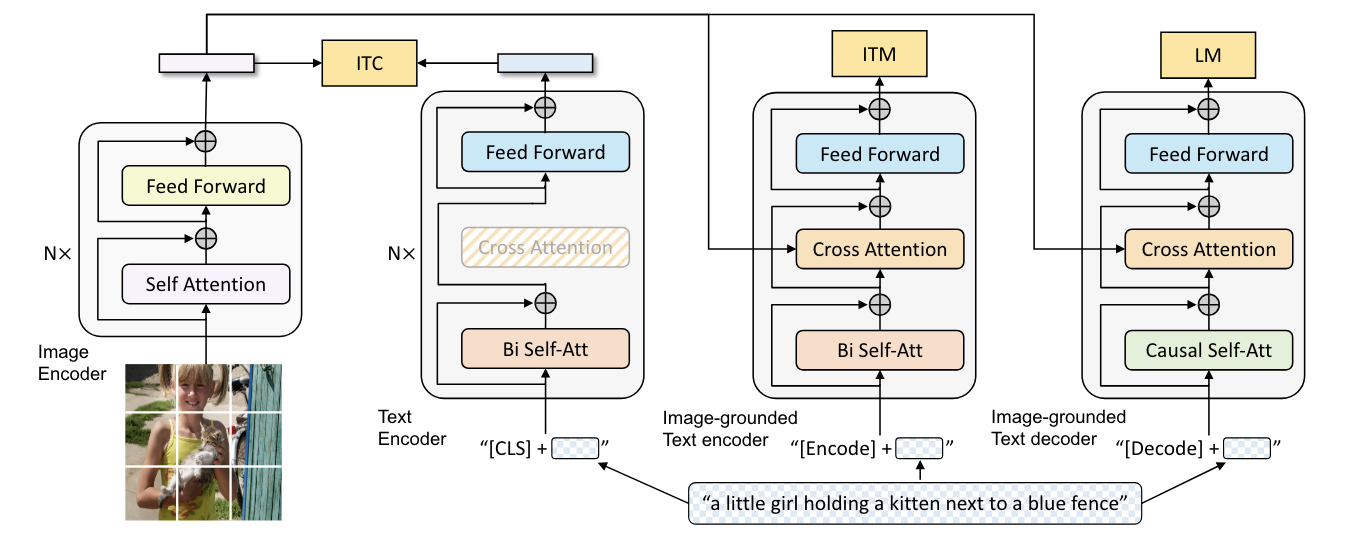
\includegraphics[width=\linewidth]{sec/Images/image2.png}
   \caption{BLIP Architecture}
   \label{fig:onecol}
\end{figure}

%-------------------------------------------------------------------------
\subsection{Wu-Palmer Similarity Score}

In paper by Malinowsk et. al \cite{malinowski2014multi} introduces a performance measure called the WUPS score for evaluating the quality of system-generated answers. It draws inspiration from Fuzzy Sets theory and utilises the Wu-Palmer Similarity (WUPS) score to account for semantic fuzziness between classes. WUPS score penalises both underestimation and overestimation of answers. The formula considers the intersection of system and ground-truth answers, employing a soft membership measure. Empirical findings suggest a WUP score of approximately 0.9 for precise answers, prompting down-weighting for scores below a threshold. A curve over thresholds illustrates the trade-off between precision and forgiveness, with WUPS at 0 being the most lenient measure and WUPS at 1.0 equating to standard accuracy. Further details about the evaluation metric will be discussed in the subsequent sections. 


%-------------------------------------------------------------------------
% \subsection{References}

% List and number all bibliographical references in 9-point Times, single-spaced, at the end of your paper.
% When referenced in the text, enclose the citation number in square brackets, for
% example~\cite{Authors14}.
% Where appropriate, include page numbers and the name(s) of editors of referenced books.
% When you cite multiple papers at once, please make sure that you cite them in numerical order like this \cite{Alpher02,Alpher03,Alpher05,Authors14b,Authors14}.
% If you use the template as advised, this will be taken care of automatically.

% \begin{table}
%   \centering
%   \begin{tabular}{@{}lc@{}}
%     \toprule
%     Method & Frobnability \\
%     \midrule
%     Theirs & Frumpy \\
%     Yours & Frobbly \\
%     Ours & Makes one's heart Frob\\
%     \bottomrule
%   \end{tabular}
%   \caption{Results.   Ours is better.}
%   \label{tab:example}
% \end{table}

% %-------------------------------------------------------------------------
% \subsection{Illustrations, graphs, and photographs}

% All graphics should be centered.
% In \LaTeX, avoid using the \texttt{center} environment for this purpose, as this adds potentially unwanted whitespace.
% Instead use
% {\small\begin{verbatim}
%   \centering
% \end{verbatim}}
% at the beginning of your figure.
% Please ensure that any point you wish to make is resolvable in a printed copy of the paper.
% Resize fonts in figures to match the font in the body text, and choose line widths that render effectively in print.
% Readers (and reviewers), even of an electronic copy, may choose to print your paper in order to read it.
% You cannot insist that they do otherwise, and therefore must not assume that they can zoom in to see tiny details on a graphic.

% When placing figures in \LaTeX, it's almost always best to use \verb+\includegraphics+, and to specify the figure width as a multiple of the line width as in the example below
% {\small\begin{verbatim}
%    \usepackage{graphicx} ...
%    \includegraphics[width=0.8\linewidth]
%                    {myfile.pdf}
% \end{verbatim}
% }


% %-------------------------------------------------------------------------
% \subsection{Color}

% Please refer to the author guidelines on the \confName\ \confYear\ web page for a discussion of the use of color in your document.

% If you use color in your plots, please keep in mind that a significant subset of reviewers and readers may have a color vision deficiency; red-green blindness is the most frequent kind.
% Hence avoid relying only on color as the discriminative feature in plots (such as red \vs green lines), but add a second discriminative feature to ease disambiguation.
\section{Dataset Description}
\label{sec:formatting}

%------------------------------------------------------------------------
We have utilized three distinct datasets to evaluate the performance of the BLIP model: VQA v2.0 Training, VQA v2.0 Validation, and the DAQUAR Dataset. Refer to Table 1 for further details.

\begin{table}[h]
\centering
\begin{tabular}{@{}lccc@{}}
\toprule
Dataset & \#Images & \#Questions & \#Answers\\
\midrule
\href{https://visualqa.org/download.html}{VQA v2.0 Training} & 82783 & 443757 & 4437570\\
\href{https://visualqa.org/download.html}{VQA v2.0 Validation} & 40504 & 214354 & 2143540\\
\href{https://www.mpi-inf.mpg.de/departments/computer-vision-and-machine-learning/research/vision-and-language/visual-turing-challenge}{DAQUAR} & 1449 & 5674 & 5674\\
\bottomrule
\end{tabular}
\caption{Comparison of \#Image, \#Question, and \#Answer Across Datasets}
\label{tab:example}
\end{table}

For the VQA v2.0 Training and Validation datasets, we were provided with 10 answers for each question. The majority is considered as the final ground truth answer. 

%-------------------------------------------------------------------------

\section{Exploratory Data Analysis}
\label{sec:formatting}

%------------------------------------------------------------------------
\subsection{Question Length Distribution Across Datasets}
The graph in Fig. 3 indicates that the majority of questions in both the training and validation sets of the VQA v2 dataset consist of 4 to 7 words, with the distributions almost overlapping, implying the validation set's representativeness of the training set. Conversely, questions in the DAQUAR dataset tend to be longer, primarily falling within the range of 6 to 11 words.

\begin{figure}[htbp]
  \centering
   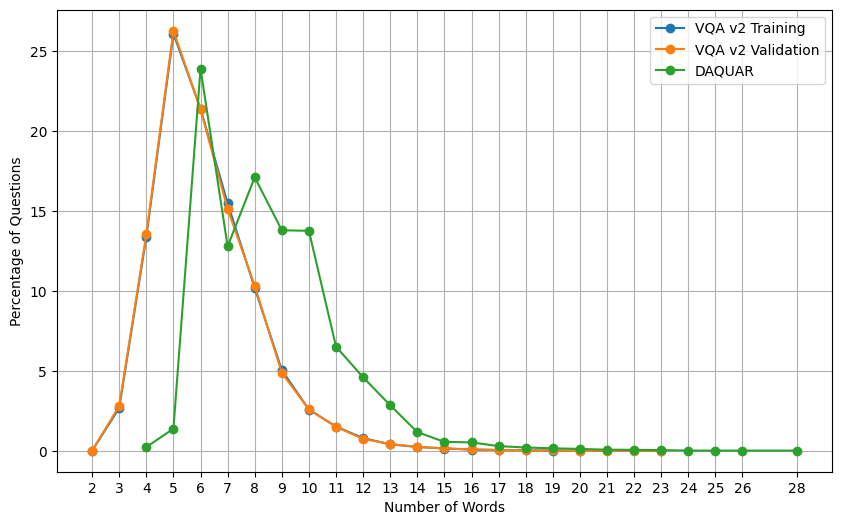
\includegraphics[width=\linewidth]{sec/Images/image3.png}
   \caption{}
   \label{fig:onecol}
\end{figure}

\subsection{Answer Length Distribution Across Datasets}
The graph in Fig. 4 reveals that the majority of answers in both the VQA v2 datasets (training and validation sets) and the DAQUAR dataset consist of 1 or 2 words. This could suggest that the questions are designed to elicit simple or direct information from the images, rather than requiring complex or elaborate explanations.

\begin{figure}[htbp]
  \centering
   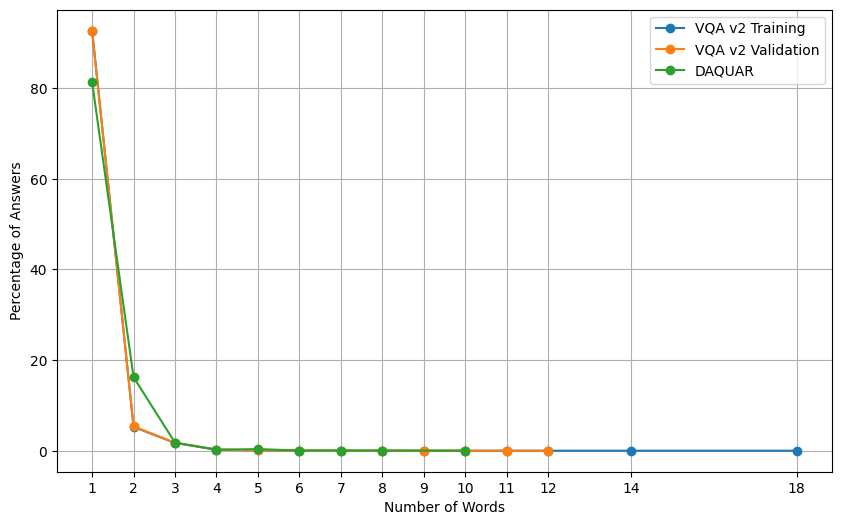
\includegraphics[width=\linewidth]{sec/Images/image4.png}
   \caption{}
   \label{fig:onecol}
\end{figure}

\subsection{Question Type Distribution Across Datasets}
The graph in Fig. 5 provides insights into the design of questions within the datasets. In the VQA v2 datasets (both training and validation sets), questions starting with “how many,” “is the,” and “what” are predominant. Conversely, in the DAQUAR dataset, questions frequently begin with “what is on the,” “what is the,” and “what is.” This suggests a focus on different types of queries in each dataset, with VQA v2 emphasising queries about quantity, state, and general attributes, while DAQUAR leans towards inquiries about object identification and description.



\begin{figure}[htbp]
  \centering
   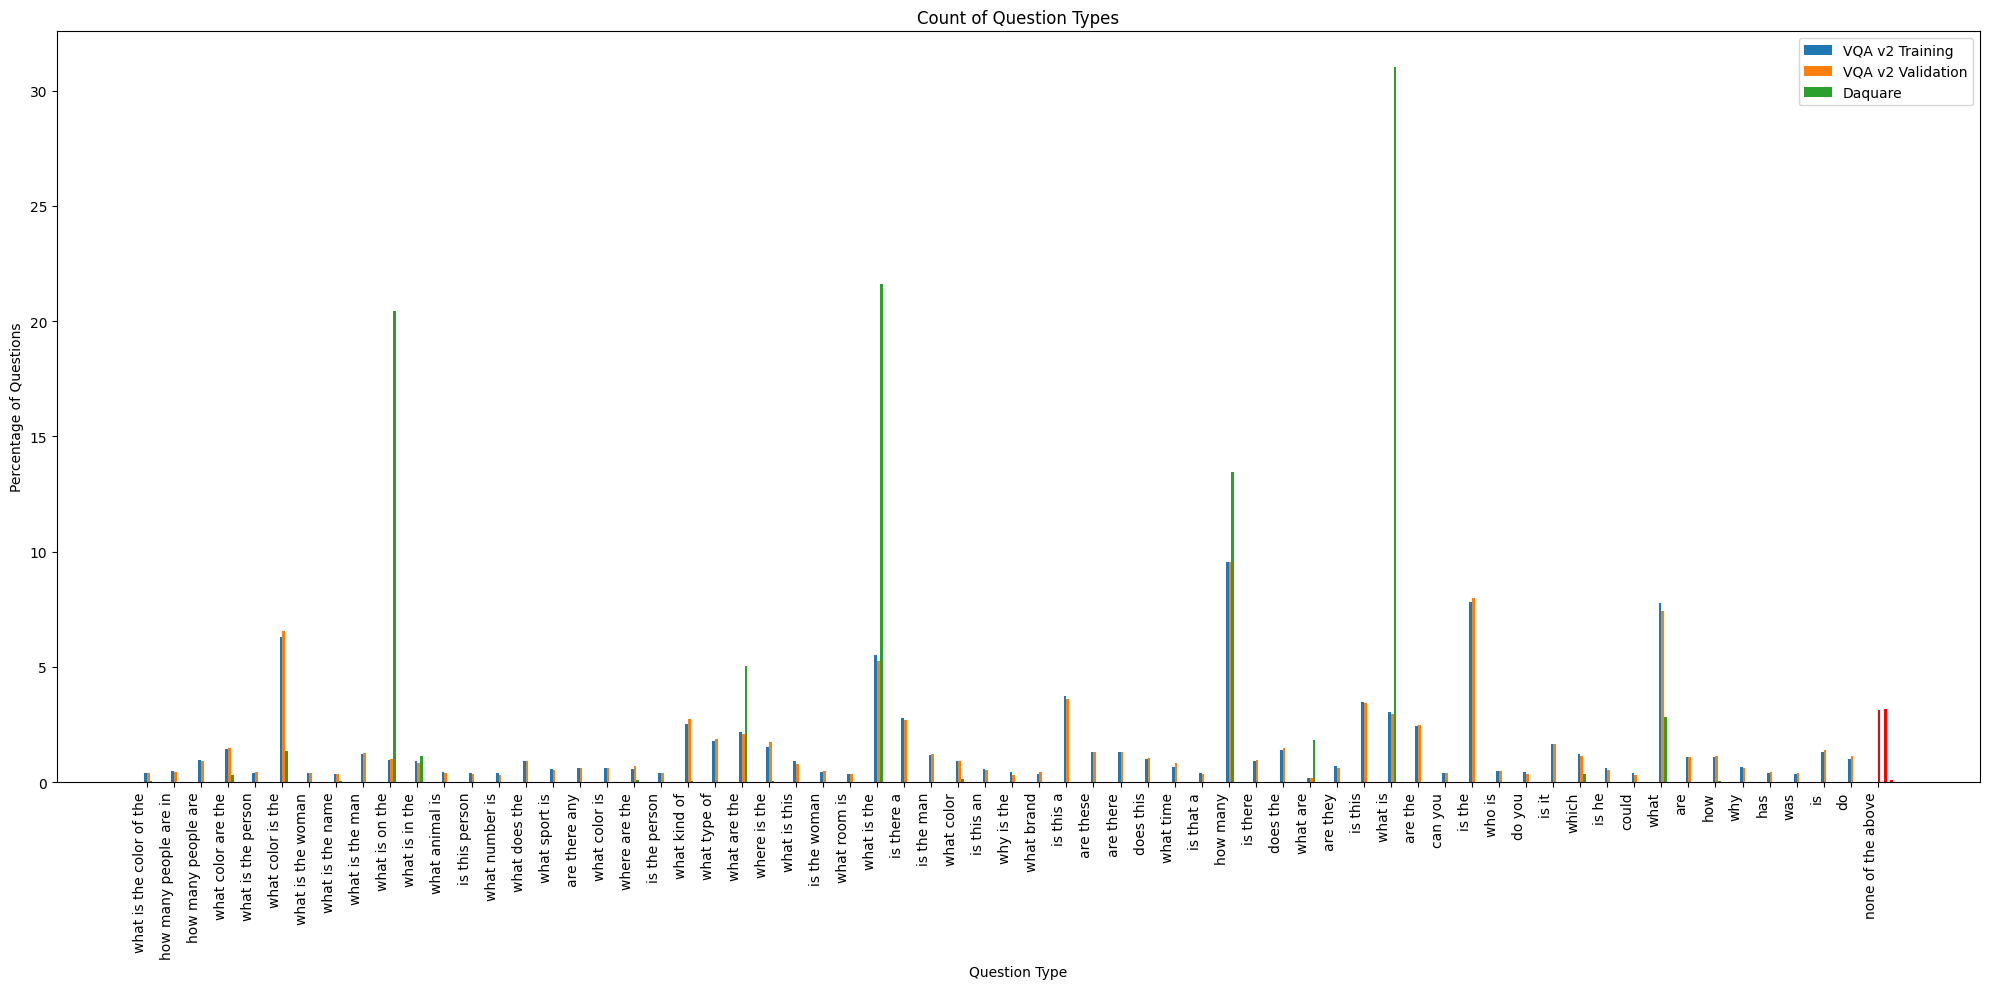
\includegraphics[width=\linewidth]{sec/Images/image5.png}
   \caption{}
   \label{fig:onecol}
\end{figure}

%-------------------------------------------------------------------------

\section{Results}
\label{sec:formatting}

%------------------------------------------------------------------------
\subsection{Accuracy}
Accuracy is the proportion of correctly predicted instances (True Positive and True Negative) out of all instances. In this an answer is correctly predicted only if it is exactly same as the ground truth answer i.e. strict matching.
    \[Accuracy = \frac{TP + TN} {TP + TN + FP + FN} \]

\begin{table}[h]
\centering
\begin{tabular}{@{}lcc@{}}
\toprule
Dataset & Accuracy\\
\midrule
VQA v2.0 Training & 0.769 \\
VQA v2.0 Validation & 0.766\\
DAQUAR & 0.230\\
\bottomrule
\end{tabular}
\caption{Accuracy Scores}
\label{tab:example}
\end{table}



\subsection{BLEU Score}
It is the geometric average of the
modified n-gram precisions, $p_{n}$, using n-grams up to
length N and positive weights $w_{n}$ summing to one.
Let c be the length of the predicted sentence and r be the ground truth sentence length. The brevity penalty BP is calculated as
\[BP= \begin{cases}1 & \text { if } c>r \\ e^{(1-r / c)} & \text { if } c \leq r\end{cases}\]
Then the BLEU score is
\[BLEU=\mathrm{BP} \cdot \exp \left(\sum_{n=1}^N w_n \log p_n\right)\].

We utilize BLEU-1, BLEU-2, BLEU-3, and BLEU-4 by respectively adjusting N and applying uniform weights $w_{n}$ = 1/N.

\begin{table}[h]
\centering
\begin{tabular}{@{}lccccc@{}}
\toprule
Dataset & BLEU1 & BLEU2 & BLEU3 & BLEU4\\
\midrule
VQA v2.0 Training &0.763&
0.552&
0.438&
0.349

 \\
VQA v2.0 Validation&0.760&
0.551&
0.438&
0.354
\\
DAQUAR &0.183&
0.081&
0.037&
0.0

\\
\bottomrule
\end{tabular}
\caption{BLEU Scores}
\label{tab:example}
\end{table}


\subsection{BERT Scores}
BERTScore leverages the pre-trained contextual embeddings from BERT \cite{devlin2018bert} and matches words in candidate and reference sentences by cosine similarity. It has been shown to correlate with human judgment on sentence-level and system-level evaluation. Moreover, BERTScore computes precision, recall, and F1 measure, which can be useful for evaluating different language generation tasks.
\begin{table}[h]
\centering
\begin{tabular}{@{}lcccc@{}}
\toprule
Dataset &BERT Pre&
BERT Rec&
BERT F1&\\
\midrule
VQA v2.0 Training &0.985&
0.986&
0.985\\
VQA v2.0 Validation&0.985&
0.985&
0.985\\
DAQUAR &0.945&
0.935&
0.939\\
\bottomrule
\end{tabular}
\caption{BERT Precision, Recall and F1 Scores}
\label{tab:example}
\end{table}


\subsection{WUPS Score}
The WUPS calculates the similarity between two words based on their
longest common subsequence in the taxonomy tree. If the similarity between two words is less than a threshold then a score of zero will be given to the candidate answer. We have
used the Wordnet \cite{miller1995wordnet} database to measure the similarity between the words. The WUPS Score is calculated using the below formula
\begin{figure}[htbp]
  \centering
   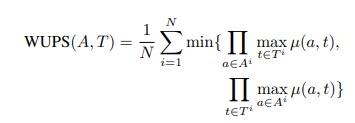
\includegraphics[width=0.7\linewidth]{sec/Images/image6.png}
   \label{fig:onecol}
\end{figure}

\begin{table}[h]
\centering
\begin{tabular}{@{}lccc@{}}
\toprule
Dataset & WUPS 0.0 & WUPS 0.9\\
\midrule
VQA v2.0 Training &
86.573&
79.484
\\
VQA v2.0 Validation&
86.223&
79.203
\\
DAQUAR &
58.122&
30.680&
\\
\bottomrule
\end{tabular}
\caption{WUPS Score at 0.0 and 0.9 Threshold}
\label{tab:example}
\end{table}

\begin{figure}[htbp]
  \centering
   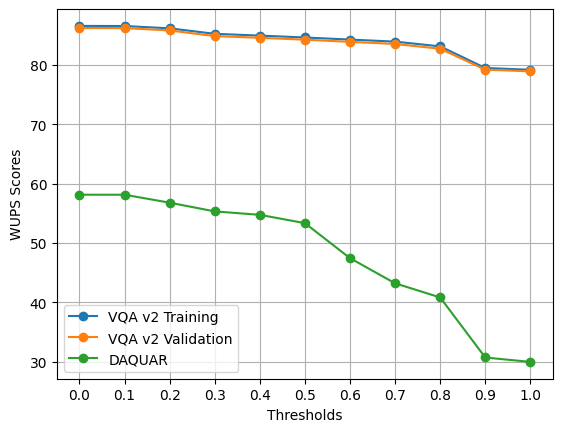
\includegraphics[width=0.75\linewidth]{sec/Images/image7.png}
   \caption{WUPS Score at different threshold}
   \label{fig:onecol}
\end{figure}

\subsection{VQA Score}
The VQA accuracy metric assesses the correspondence between the model's response and all potential answers provided for a given question. If the model's response matches exactly with a minimum of three among the available answers, the VQA accuracy is rated as 1; otherwise, it falls below 1. To evaluate this metric, multiple answers to a question are required. However, since we don't have that in the DAQUAR dataset, we haven't calculated it for this.

% \begin{figure}[htbp]
%   \centering
%    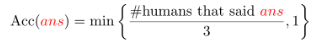
\includegraphics[width=\linewidth]{sec/Images/image8.png}
%    \label{fig:onecol}
% \end{figure}

\[Acc(ans)=\min \left\{\frac{\text { \#humans that said ans }}{3}, 1\right\}\]

\begin{table}[h]
\centering
\begin{tabular}{@{}lcc@{}}
\toprule
Dataset & VQA Score\\
\midrule
VQA v2.0 Training &
84.89
\\
VQA v2.0 Validation&
84.73
\\
DAQUAR &
--
\\
\bottomrule
\end{tabular}
\caption{VQA Scores}
\label{tab:example}
\end{table}


%-------------------------------------------------------------------------

\section{Experimental Setup}
\label{sec:formatting}
Since the VQA v2.0  dataset was very large (approximately 82,000 in the training dataset), we divided it into 10 parts and split these parts among the 3 members to achieve parallelisation. We used the BLIP model for each part and then combined the outputs for all the parts to evaluate the results.
For the validation set of VQA v2 we divided it into 2 parts and combined the outputs for both parts to evaluate the results.
DAQUAR dataset was not large (approximately 1500 images), so we did not divide it into parts.

%------------------------------------------------------------------------






\section{Analysis}
\label{sec:formatting}
In this section we will go through the drawbacks and advantages of the evaluation metric with the help of two question-answer pairs projected on the same image. 
\begin{figure}[htbp]
  \centering
   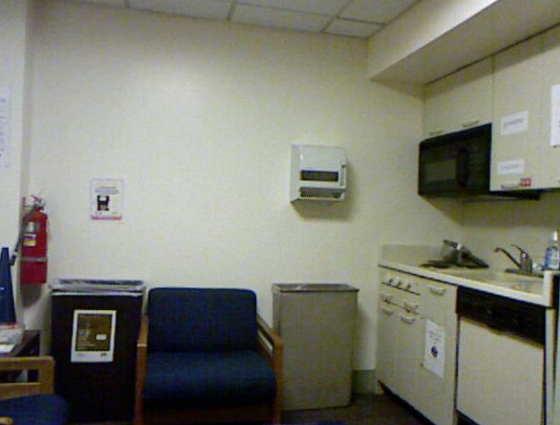
\includegraphics[width=0.75\linewidth]{sec/Images/image9.png}
   \caption{}
   \label{fig:onecol}
\end{figure}



Fig. 7 shows an image instance from DAQUAR dataset to which the BLIP question-answer model is applied. 
Fig. 8 presents two cases which includes the question asked, the prediction we get and the ground truth on the image.

\begin{figure}
    \centering
    \begin{subfigure}{0.5\textwidth}
        \centering
        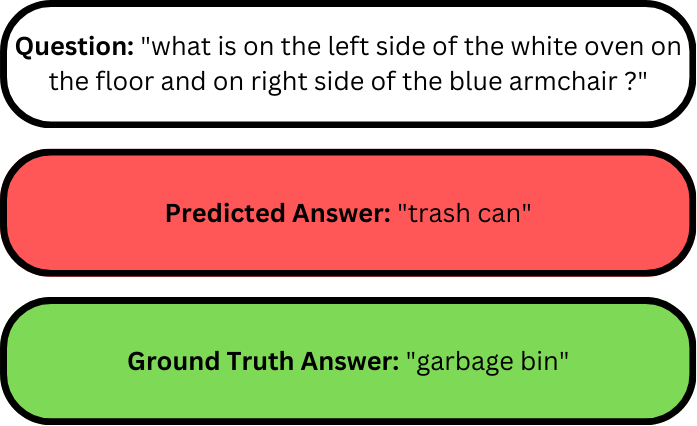
\includegraphics[width=0.5\textwidth]{sec/Images/image10.png}
        \caption{Case 1}
        \label{fig:sub1}
    \end{subfigure}
    \hfill
    \begin{subfigure}{0.5\textwidth}
        \centering
        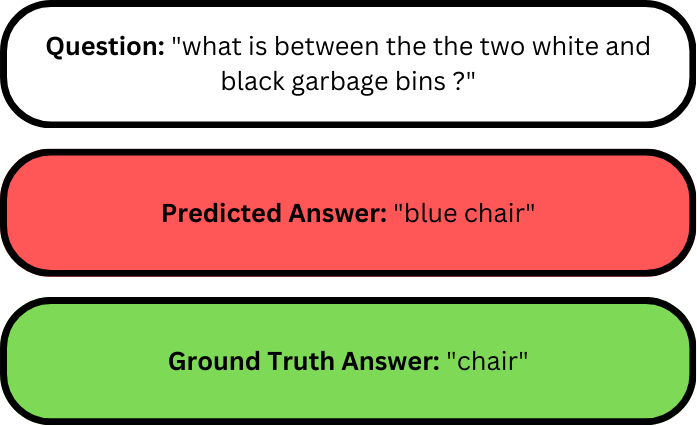
\includegraphics[width=0.5\textwidth]{sec/Images/image11.png}
        \caption{Case 2}
        \label{fig:sub2}
    \end{subfigure}
    \label{fig:whole}
\end{figure}


\subsection{Accuracy}
As evident from the results, the BLIP model exhibits relatively low accuracy. However, relying solely on accuracy metrics may not comprehensively assess the model's performance. As shown in the example above, strict matching between predicted and best ground truth results may overlook semantically similar answers, as explained below : \\
\begin{itemize}
    \item \textbf{Case 1}: The model predicted "trash can" while the ground truth was "garbage bin", resulting in a 0 accuracy score despite the similarity in meaning.
    \item \textbf{Case 2}: The model predicted "blue chair" while the ground truth was "chair", resulting in a 0 accuracy score despite the more detailed answer.
\end{itemize}


Hence, accuracy alone may not adequately reflect the model's effectiveness in capturing nuanced semantic relationships.

\subsection{BLEU Score}

The BLIP model's subpar accuracy underscores the importance of adopting nuanced evaluation metrics such as the BLEU score. Unlike traditional accuracy, BLEU considers n-gram overlaps, providing a more comprehensive understanding of the model's performance across diverse datasets.

\begin{itemize}
    \item \textbf{Case 1}: The model predicted "trash can" while the ground truth was "garbage bin", resulting in a 0 BLUE score despite the similarity in meaning because it checks for the n-gram overlaps.
    \item \textbf{Case 2}: The model predicted "blue chair" while the ground truth was "chair", resulting in a 0.5 BLUE score due to a small degree of overlap in the answer.
\end{itemize}

Thus, the BLUE score is better than the standard accuracy but is still insufficient because it does not take the semantic similarity into account.


\subsection{BERT Score}
\begin{itemize}
    \item \textbf{Case 1}: The model achieved a BERT Precision score of 0.90, indicating high semantic similarity between the model’s output (“trash can”) and the ground truth value (“garbage bin”).
    \item \textbf{Case 2}: The model predicted "blue chair" while the ground truth was "chair", resulting in a BERT Precision score of 0.83 due to high similarity.
\end{itemize}

Thus, as shown by the results, the BERT score is a highly valuable metric for assessing the performance of the model.

\subsection{WUPS Score}
\begin{itemize}
    \item \textbf{Case 1}: The WUPS score is good in case 1. The score is 0.76 at 0 threshold and 0.0076 at 0.9 threshold.
    \item \textbf{Case 2}: The WUPS does not provide a good score in case 2. The score is 0.11 at 0 threshold and is 0.011 at 0.9 threshold.
\end{itemize}

WUPS score provides us insight into the semantic similarity between our model’s output and the ground truth values in some cases, however, it is unable to capture the semantic similarity of the words in all the cases. 

\subsection{VQA Accuracy}
\begin{itemize}
    \item \textbf{Case 1}: VQA accuracy is 0.67 because the model’s output matched 2 answers out of the 10 available answers.
    \item \textbf{Case 2}: VQA accuracy is 0.33 because the model’s output matched exactly 1 answer of the 10 available answers.
\end{itemize}

VQA score provides a more accurate depiction of the model’s performance as compared to simple accuracy by comparing the predictions with all the available answers. However, it still does not take the semantic similarity into account, which is not ideal. 
%------------------------------------------------------------------------






\section{Commentary}
\label{sec:formatting}

\subsection{Ritwik Harit}
Through our study, we have used a comprehensive framework to evaluate the performance of the BLIP model across different datasets. We have conducted a detailed exploratory data analysis to showcase the datasets and their characteristics. Moreover, the Results and Analysis section highlights the areas where our model performs well and where it needs improvement. As shown by poor accuracy on the DAQUAR dataset, the BLIP model is unable to predict the exact answers in many cases. However, the high BERT scores show that there is a high degree of semantic similarity between the predictions of the BLIP model and the ground truth answers. Such specialised metrics for evaluation provide us with better insights into the performance of the model, which have not been used in the original paper.
\subsection{Shreyas Kabra}
Our task was to evaluate the performance of the BLIP model across different datasets including the one it was trained on. As shown by the results, the model performs exceptionally well for the VQA v2 dataset, however, its performance decreases sharply on the DAQUAR dataset. However, the value of the BERT score is still very good on the DAQUAR dataset, implying that the model is able to produce results which are semantically similar to the ground truth. Moreover, good results on the VQA datasets suggest that the model is trained well and gives precise results for these datasets, as shown by high accuracy. However, such precision is lost when the DAQUAR dataset is used, as shown by the low accuracy score. 
\subsection{Vasan Vohra}
In this project, we looked at how to utilize BLIP on different datasets to bring out the best outcomes in the VQA, i.e., Visual Question Answering. The task is to extract an answer from a given image based on the question provided. The first step was an extensive dataset analysis to understand the features. The next step is to understand the different metrics that could be utilized to evaluate the results. We have provided an explanation of why a particular metric is better than another. The low accuracy and BLEU score in DAQUAR make it clear that the model cannot give exact answers. The high BERT score in the same means that the meaning of the outcomes of the BLIP is closer to the result we need to reach. The overall results on the VQA dataset were better than DAQUAR. Using better and more explanatory evaluations in the model outputs makes this project different from the already defined papers.


%------------------------------------------------------------------------






{
    \small
    \bibliographystyle{ieeenat_fullname}
    \bibliography{main}
}

% WARNING: do not forget to delete the supplementary pages from your submission 
% \clearpage
\setcounter{page}{1}
\maketitlesupplementary


\section{Rationale}
\label{sec:rationale}
% 
Having the supplementary compiled together with the main paper means that:
% 
\begin{itemize}
\item The supplementary can back-reference sections of the main paper, for example, we can refer to \cref{sec:intro};
\item The main paper can forward reference sub-sections within the supplementary explicitly (e.g. referring to a particular experiment); 
\item When submitted to arXiv, the supplementary will already included at the end of the paper.
\end{itemize}
% 
To split the supplementary pages from the main paper, you can use \href{https://support.apple.com/en-ca/guide/preview/prvw11793/mac#:~:text=Delete%20a%20page%20from%20a,or%20choose%20Edit%20%3E%20Delete).}{Preview (on macOS)}, \href{https://www.adobe.com/acrobat/how-to/delete-pages-from-pdf.html#:~:text=Choose%20%E2%80%9CTools%E2%80%9D%20%3E%20%E2%80%9COrganize,or%20pages%20from%20the%20file.}{Adobe Acrobat} (on all OSs), as well as \href{https://superuser.com/questions/517986/is-it-possible-to-delete-some-pages-of-a-pdf-document}{command line tools}.

\end{document}
